\documentclass[10pt,preprint]{sigplanconf}

\usepackage[utf8]{inputenc}
% the following standard packages may be helpful, but are not required
%\usepackage{longtable}
\usepackage{mathtools}
\usepackage{multicol}
\usepackage{multirow}
\usepackage{booktabs}
\usepackage{courier}
\usepackage[scaled]{helvet}
\usepackage{url}
\usepackage{listings}
\usepackage{enumitem}
\usepackage{mdwlist} % tighter description environment (starred)
\usepackage[colorlinks=true,allcolors=blue,breaklinks,draft=false]{hyperref}
% known bug: http://tex.stackexchange.com/questions/1522/pdfendlink-ended-up-in-different-nesting-level-than-pdfstartlink
\newcommand{\doi}[1]{doi:~\href{http://dx.doi.org/#1}{\Hurl{#1}}}   % print a hyperlinked DOI

\usepackage{graphicx}
\usepackage{softdev}
\usepackage{amsmath}
\usepackage{mdwlist}
\usepackage{pifont}
\usepackage{xspace}

\newcommand{\kalibera}{Kalibera \& Jones\xspace}
\newcommand{\krun}{Krun\xspace}
\newcommand{\hypone}{H1\xspace}
\newcommand{\hyptwo}{H2\xspace}
\newcommand{\binarytrees}{\emph{binary trees}\xspace}
\newcommand{\richards}{\emph{Richards}\xspace}
\newcommand{\spectralnorm}{\emph{spectralnorm}\xspace}
\newcommand{\nbody}{\emph{n-body}\xspace}
\newcommand{\fasta}{\emph{fasta}\xspace}
\newcommand{\fannkuch}{\emph{fannkuch redux}\xspace}
\newcommand{\bencherthree}{4709K/Linux\xspace}
\newcommand{\bencherfive}{4790/Linux\xspace}
\newcommand{\benchersix}{4790/OpenBSD\xspace}
\newcommand{\bencherseven}{ARM\xspace}

\lstset{
    basicstyle=\tt\scriptsize,
    xleftmargin=2em,
    framexleftmargin=1.5em,
    numberstyle=\scriptsize\tt\color{gray},
    captionpos=b,
    escapeinside={{<!}{!>}},
}

\begin{document}

\title{Virtual Machine Warmup Blows Hot and Cold}
\authorinfo{Edd Barrett}
           {Software Development Team\\ Department of Informatics\\ King's College London}
           {http://eddbarrett.co.uk/}
\authorinfo{Carl Friedrich Bolz}
           {Software Development Team\\ Department of Informatics\\ King's College London}
           {http://cfbolz.de/}
\authorinfo{Rebecca Killick}
           {Department of Mathematics and Statistics\\ University of Lancaster}
           {http://www.lancs.ac.uk/\~{}killick/}
\authorinfo{Vincent Knight}
           {School of Mathematics\\ Cardiff University}
           {http://vknight.org/}
\authorinfo{Sarah Mount}
           {Software Development Team\\ Department of Informatics\\ King's College London}
           {http://snim2.org/}
\authorinfo{Laurence Tratt}
           {Software Development Team\\ Department of Informatics\\ King's College London}
           {http://tratt.net/laurie/}
\maketitle

\begin{abstract}
Warmup is magic.
\end{abstract}

\section{Introduction}
\label{sec:intro}

\laurie{we need a really simple graph in the intro, along the lines of the one
in the glowworm proposal. and not the current figure 1, whose caption is really
confusing!}

\laurie{since, at the moment, we don't say anything about how \emph{long} it
takes to warmup, i've not tried saying at all about that.}

Many modern languages are implemented as Virtual Machines (VMs) which use a
Just-In-Time (JIT) compiler to translate `hot' parts of a program into efficient
machine code at run-time. Since it takes time to determine which parts of the
program are hot, and then compile them, programs which are JIT compiled are
said to be subject to a \emph{warmup} phase. The traditional view of
JIT compiled VMs is that program execution is slow during the warmup phase, and
fast afterwards, when \emph{peak performance} is said to have been reached.
This traditional view underlies most benchmarking of JIT compiled VMs, which
generally aim to measure peak performance. Benchmarking methodologies usually
require running benchmarks several times within a single VM process, and
discarding any timing data collected before warmup is complete.

Our fundamental aim in this paper is to test the following hypothesis, which captures a constrained
notion of the traditional notion of warmup:
\begin{description}
  \item[\hypone] Small, deterministic programs exhibit traditional warmup behaviour.
\end{description}
In order to test this hypothesis, we present a carefully designed
experiment where a number of simple benchmarks are run on a variety of
VMs for a large number of in-process iterations and repeated using fresh
processes. From this we obtain \emph{time series} data, to which we apply a
number of statistical techniques that have not previously been applied
in the context of VM benchmarking.

\begin{figure}[b!]
\centering
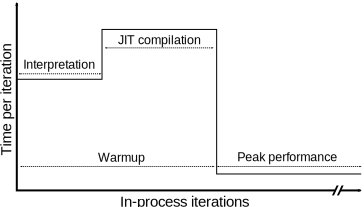
\includegraphics[width=.4\textwidth]{img/picturebook_warmup}
\caption{The traditional notion of warmup: a program starts slowly executing in
an interpreter; once hot parts of the program are identified, they are
translated by the JIT compiler to machine code; at this point warmup
is said to have completed, and peak performance reached.}
\label{fig:trad}
\end{figure}

We expected our experiment to validate Hypothesis H1, allowing us to
easily compare warmup across VMs. While some benchmarks on some VMs run as per
traditional expectations, we found a number of surprising cases. At
the most extreme, some benchmarks never warmup, staying at their initial performance
levels indefinitely and some `warmdown', getting slower over time. Even for
those benchmarks that appear to warmup in a traditional fashion, there are
various performance patterns that make presenting a simple performance number
difficult. Of the eight VMs we looked at,
none consistently warmed under the traditional model \edd{check this is true
when we have all the results}.

Our results thus suggest that the traditional view of warmup is badly out of date. 
We suggest it is better to think of most benchmarks as
generally converging on a \emph{steady state} of performance (be that faster or
slower than initial execution). When a benchmark does not converge on a steady
state, we suggest that it is impossible to give meaningful performance figures.
We believe our results are of interest to VM writers, but also to users of
those VMs. Authors may not have considered the different types of warmup
behaviour (or found benchmarks which trigger such behaviour), whereas users may
obtain a greater understanding of why their programs do not perform as well as
they had expected.

This paper's contributions are as follows:
\begin{enumerate*}
  \item \laurie{blah blah}
\end{enumerate*}

This paper's structure is as follows. \laurie{blah blah}


\section{Background}
\label{sec:warmup}

When a program begins running on a JIT compiled VM, it is typically (slowly)
interpreted; once `hot' (i.e.~frequently executed) loops or methods are
identified, they are dynamically compiled into machine code; and subsequent
execution of those loops or methods uses (fast) machine code rather than the
(slow) interpreter. Once machine code generation has completed, the VM is
traditionally said to have finished warming up, and the program to be executing
at peak performance.\footnote{This traditional notion applies equally to VMs
that perform immediate compilation instead of using an interpreter, and to
those VMs which have more than one layer of JIT compilation (later JIT
compilation is used for `very hot' portions of a program, and tolerates slower
compilation time for better machine code generation).}

Figure~\ref{fig:trad} shows the expected performance profile of a
program subject to the conventional model of warmup. Exactly how long warmup
takes is highly dependent on
the program and the JIT compiler, but this basic assumption about the
performance model is shared by every JIT compiling
VM~\cite{kalibera13rigorous}.

Benchmarking of JIT compiled VMs typically focusses on peak
performance.\footnote{There are various cultural and technical reasons for this,
ranging from the difficulty of determining warmup, to the flattering effect that
peak performance can imbue on programs that are JIT compiled.} The
methodologies used are typically crude. Benchmarks are run for a number of
iterations within a single VM process, with timing data for each iteration
recorded. The first $n$ iterations are then discarded, on the basis that warmup
will have completed before these $n$ iterations have finished. It is common for
a hard-coded number to be used for $n$ (in our experience, it is often set at 5)
to be used for all benchmarks.

One of the obvious flaws in this simple methodology is that one does not know if warmup
has completed by iteration $n$. A more sophisticated VM benchmarking methodology
was developed by \kalibera to solve a number of issues when benchmarking JIT
compiling VMs~\cite{kalibera12quantifying,kalibera13rigorous}. The basic idea is
that, for a given VM / benchmark combination, a human must inspect the data from
executing a small number of VM processes, and determine at which iteration the
benchmark has definitively warmed up. A larger number of VM processes are then
run, and the previously determined cut-off point applied to each process's
iterations. The \kalibera methodology observes that some benchmarks do not
obviously warmup \laurie{this is not reaching the `independent' state, right?
what happens to such benchmarks? do \kalibera say ``you can't do anything with
such benchmarks'' or ...?}\cfbolz{there are two states according to Kalibera:
"initialized" and "independent". Initialized means that the results start
looking stable at some point, and the weird behaviour of the prefix is removed.
Independent is always stronger than initialized, and means that the results
start being statistically independent from each other. Kalibera seem to assume
that every benchmark eventually initializes (and indeed I think one of our
results should be that that is not obviously true). If a benchmark also becomes
independent, their full methodology applies. If it does not, their suggestion
is to always pick as a result a fixed iteration. So another of our results is
that that is also not a good suggestion, because of cyclic behaviour.}; and
that others follow cyclic patterns post-warmup
(e.g.~iteration $m$ is slow, $m+1$ is fast, for all even values of $m > n$). In
the latter case, the \kalibera methodology requires a consistent iteration in
the cycle to be picked, and that used for statistical analysis.

To the best of our knowledge, the \kalibera methodology is the most
sophisticated currently available, and has been used by other authors (see
e.g.~\cite{barrett15approaches,grimmer15dynamically}). While the \kalibera
methodology is a real improvement over crude benchmarking methodologies,
our experience has been that there remain cases where it remains hard to produce
satisfying benchmarking statistics. Crucially, the methodology does not
provide a firm way of determining when warmup has completed. Because of this
``determining when a system has warmed up, or even providing a
rigorous definition of the term, is an open research problem''~\cite{seaton15phd}.


\section{Methodology}
\label{sec:methodology}

To test Hypothesis H1, we designed an experiment with a simple basic idea: to
take a number of micro-benchmarks derived and
run them in a loop of 2000 iterations on a number of VMs. We repeat this
process 10 times before analysing the resulting time series data. In order
that we the data we obtain high-quality data, we have carefully designed our
experiment to be repeatable and to control as many potentially confounding variables as
is practical.

In this section we detail our methodology: the benchmarks we use and the
modifications we made to them; the machines we used for benchmarking; the VMs we
benchmarked; and the \krun system we developed to run benchmarks.


\subsection{The Micro-benchmarks}

The micro-benchmarks we use are as follows: \binarytrees, \spectralnorm, \nbody,
\fasta, and \fannkuch from the Computer Language Benchmarks Game (CLBG); and
\richards. For each benchmark, we provide C, Java, Javascript, Python, Lua, PHP,
and Ruby versions.\footnote{Our need to have implementations in a wide variety
of languages restricted the micro-benchmarks we could use.} Since most of these
benchmarks have multiple implementations in any given language, we mostly picked
the same versions used in~\cite{bolz14impact}, which represented the fastest
performers at the point of that publication. In a few cases \laurie{can we say
``X of Y'' i.e. something like ``about 3 of 40 benchmarks''?}, we noted that
substantially faster implementations are now available, and substituted them
accordingly.

Readers can be forgiven for initial scepticism about this set of micro-benchmarks.
They are small and widely
used by VM authors as optimisation targets. In general they are more effectively
optimised by VMs than average programs; when used as a proxy for other types
of programs (e.g.~large programs), they tend to overstate the effectiveness of
VM optimisations. In our context, this weakness is in fact a strength: we need
small, deterministic, and widely examined programs so that we can test
Hypothesis \hypone. Put another way, if we were to run arbitrary programs
and find unusual warmup behaviour, a VM author might reasonably counter that
``you have found the one program that exhibits unusual warmup behaviour''.

Each benchmark was run for \laurie{XXX} executions, each comprising 2000
iterations. For the avoidance of doubt -- and in
contrast to some other experiments we are aware of \laurie{can we cite?} -- we 
did not interfere with any VMs Garbage Collection (GC) (e.g.~we did not
force a collection after each iteration).


\subsubsection{Ensuring Determinism}

We wished to ensure, as far as possible, that the micro-benchmarks are
deterministic from the user's perspective, by which we mean that they
take precisely the same path through the Control Flow Graph (CFG) on each
execution and iteration. Note that this definition deliberately focuses
on non-determinism that is controllable by the user; other forms of
non-determinism within the VM are deliberately excluded, as they are
part of what we are trying to measure (e.g.~objects in memory may be allocated
or garbage collected non-deterministically). To test this, we created variants
of all benchmarks with \texttt{print} statements at all possible points of
divergence (e.g.~\texttt{if} statements' true and false branches).\footnote{These
variants are available in our experimental suite.}

We first ran the benchmarks many \edd{how many?} times, and compared the outputs
of different runs. This showed that the \fasta benchmark was non-deterministic
in all language variants. \fasta generates random numbers using a simple
algorithm. The random seed was initialised at the start of \fasta, but not after
each iteration, so each iteration generated different random numbers. We thus
moved the random seed initialisation to the benchmark's main loop, ensuring that
each iteration uses the same sequence of random numbers.

Bearing in mind surprising
results such as the importance of link order~\cite{mytkowicz09surprising}, we
then used two different machines to compile VMs and then ran the benchmarks
on these machines. \laurie{CF: please check to see if
the remainder of this paragraph is right} This showed that the Java class loader
initialises classes in a non-deterministic order, which affected the way that
some parts of Java benchmarks were executed in \laurie{as I wrote that, I became
aware that I don't really understand why this source of non-determinism crept
into our benchmarks. Was it inside the main loop? If so, how?} \laurie{i now
think the problem is that classes are loaded lazily as they are used, though i
admit i'm not sure how our nondeterminism checks spotted this}.\edd{As I
understand it, that is not a compile-time effect, but a run-time effect? Maybe
expand/reword}\cfbolz{the story of the java class loader had nothing at all to
do with the need for different machines, imo. what happened originally was: the
benchmark class was loaded in the first iteration, which meant that most of the
time of the first iteration was spent doing class loading (file reads, security
checks, etc). now I wrote code to make sure that the benchmark classes are
loaded ahead of the first iteration, which solves the problem entirely. class
loading is actually pretty deterministic, as long as there are no wildcards in
the CLASSPATH env var.}


\subsubsection{Measuring Computation and Not File Performance}

Micro-benchmarks perform computation which is not then used. Highly optimising
compilers notice this, and can often optimise away part or all of a
micro-benchmark's computation. To avoid this happening, most micro-benchmarks
output intermediate and final results to \texttt{stdout} so that computation is
not optimised away. However, one can quickly end up in a situation where one is
unintentionally measuring, in part or whole, the performance of file routines in
the OS libraries and the kernel.

To lessen the possibility of optimising compilers removing benchmark computation,
we modified all of the benchmarks to calculate a checksum on each iteration
\laurie{i assume we output the final checksum to stdout, otherwise a clever
compiler might manage to remove everything. or do we add all the checksums
together so that we can guarantee the optimiser in fact runs every
iteration?}\cfbolz{we compared the checksum against the expected checksum and
if that fails, we print. Imo that makes it very hard for the compiler to remove
the checksum code.}.
At the end of each iteration, the checksum is validated against an expected
value. Note that each micro-benchmark has a single checksum value for all
language variants, which provides some assurance that each language variant is
performing the same work.


\subsection{Benchmarking Machines}

We used three machines and two operating systems:
\begin{description*}
  \item[\bencherthree] A quad-core i7-4790K 4GHz machine with 24GB of RAM, running Debian 8.
  \item[\bencherfive] A quad-core i7-4790 3.6GHz machine with 32GB of RAM, running Debian 8.
  \item[\benchersix] Identical hardware to \bencherfive, but running OpenBSD 5.8.
\end{description*}
These machines allow us to investigate the effects of moderately different
hardware (\bencherthree and \bencherfive run the same operating system with the
same updates installed) as well as moderately different operating systems
(\bencherfive and \benchersix have almost identical hardware, but run different
Unix
variants). With regards to hardware and operating systems, we started with the
following hypothesis:
\begin{description}
  \item[\hyptwo] Moderately different hardware and operating systems have little effect on warmup patterns.
\end{description}
We deliberately use the word `moderately', since significant changes of hardware
(e.g.~x86 vs.~ARM) or operating system (e.g.~Linux vs.~Windows) implies that
significantly different parts of the VMs will be used (e.g.~different machine
code backends may be of differing levels of maturity).

On Intel machines, we disabled turbo boost and hyper-threading in the BIOS. Turbo boost is a
feature which allows CPUs to temporarily run in an extremely high-performance
mode; this eventually causes the CPU to exceed its safe thermal limit, and
performance is then reduced to a lower limit. Turbo boost can thus cause long-running processes to
appear to suddenly slow down. Hyper-threading gives the illusion that a single
physical core is in fact more than one core, allowing more programs to
run semi-simultaneously. However, hyper-threading causes programs to interfere
with each others in complex ways, introducing considerable noise\edd{cite?}. It
is of no real benefit in our situation, where we do not make use all of the
physical cores in our benchmarking machines.


\subsection{VMs under investigation}

We ran the benchmarks on the following VMs:
\begin{description*}
\item[GCC] On Linux systems, version 4.9.2 from Debian packages; on OpenBSD the base version 4.2.1.
\item[CPython 2.7.10] The reference Python implementation\laurie{not currently, right?}.
\item[Graal \#9dafd1dc5ff9] Oracle's next-gen VM targeting Java.
\item[HHVM 3.7.1] Facebook's PHP JIT.
\item[JRuby/Truffle \#7f4cd59cdd1c8] A Ruby interpreter using Graal for dynamic compilation.
\item[HotSpot 8u45b14] The most widely used Java VM.
\item[LuaJIT 2.0.4] A tracing JIT for Lua.
\item[PyPy 4.0.0] A meta-tracing VM for Python-2.7.
\item[V8 4.8.271.9] Google's JIT for Javascript.
\end{description*}
Although not a VM, GCC serves as a baseline to compare the VMs against.

We created a build script which downloads, configures, and builds all of the
VMs, ensuring we can easily repeat builds.
On Debian all VMs were compiled with GCC/G++ \laurie{version number}. On OpenBSD,
most VMs were compiled with GCC 4.2.1, except for PyPy, HotSpot, and V8 where
GCC 4.9.3 was used.\footnote{In a future version of this paper, we will use a
single C compiler for all operating systems and all VMs.} Neither HHVM nor
JRuby/Truffle has currently been ported to OpenBSD, and thus we were unable to
run those VMs on OpenBSD.


\subsection{\krun}

We developed a tool, called \krun, to fully automate the running of benchmarks
and control the environment that benchmarks are run in. \krun itself is a
`supervisor' process which first configures a system before running VM-specific
benchmarks, monitoring the system for any signs of errors during benchmarking,
and writing results to a JSON file. \krun is invoked with a configuration file
which describes the VMs, benchmarks, and number of executions and iterations to
be executed. \krun is a generic tool, with utility beyond this paper, though
here we discuss only the parts relevant to this paper's experiment. 

In the rest
of this subsection, we describe: the variables which \krun controls, both
platform neutrally and platform specific; and how it collects iterations data.
Note that, although \krun has modes in which various checks are disabled, we
describe only the `full run' mode in which such checks are enforced.


\subsubsection{Platform Independent Controls}

Several of \krun's operations work on all supported platforms. \krun imposes a
consistent heap (we set 2GiB) and stack (we set 8MiB) \texttt{ulimit} for each
VM (we used a 2GiB heap and a 8MB stack).\footnote{Note that Linux allows users
to inspect these values, but to allocate memory beyond them.} Benchmarks are run
as a specific Unix user `\texttt{krun}' with a fresh environment. When run in
`production' mode, \krun reboots the system before each benchmark (including
before the first benchmark) to ensure that the system is in a known state
(e.g.~if a benchmark caused a system to transfer memory to disk-based swap,
rebooting ensures that later benchmarks are not affected). After reboot, \krun
is run from \texttt{/etc/rc.local}; it pauses for 3 minutes to allow the system
to fully initialise before running the next benchmark.

\krun performs two types of monitoring before and during benchmark execution.

First, \krun monitors the system's \texttt{dmesg} buffer, informing the user of
any changes \laurie{did we ever implement the `ignore unimportant changes'
thing?}. We implemented this feature after noticing that one of the machines we
earlier ear-marked for running benchmarks occasionally overheated, throttling
performance, leaving only a single line in the \texttt{dmesg} to inform us; as
readers will no doubt hope, we did not use this machine for our final
benchmarking.

Second, \krun monitors CPU temperature. Since modern CPUs downgrade their
performance when they get too hot, \krun
ensures that benchmarks start with the CPU at (approximately) the same target.
When initially invoked, \krun reads the temperatures of all available CPU cores
\laurie{or just one? does it pause before taking this reading?}. Before running
further benchmarks, it then waits for the CPU to cool down to within 10\%{} of
the starting CPU core temperatures. If the system fails to cool down to within
this threshold in 10 minutes, \krun terminates the entire experiment. Note that
since \krun has no way of knowing what a `cool' temperature is in advance, for
this feature to be fully effective, \krun assumes that the machine is adequately
cool when first invoked.


\subsubsection{Linux-specific Controls}

On Linux, \krun enables several additional factors to be controlled.

\krun sets the CPU frequency to the highest possible non-over-clocked value
(without over-clocking). This is achieved by disabling Intel P-state support in
the kernel \laurie{how?} and setting the CPU governor to \texttt{performance} mode.

\krun checks that Linux's boot-time \texttt{isolcpus} argument has been set to
remove one or more CPU cores from having processes scheduled on them. If a CPU
core has been isolated, \krun \laurie{automatically?} schedules benchmarks to be
run on that core. This means that the benchmarks are not preemptively context
switched, which can have unpredictable effects on performance. \krun also checks
that it is running on a `tickless' kernel. By default, Linux's kernel queries
each CPU 1000 times per second (the `ticks') to determine which processes are
currently running \laurie{is this per core or per CPU?}. This repeated querying
interferes with process execution, but is of little use in our setup where only
a minimal number of non-benchmarking processes are running.

Linux's \texttt{perf} system dynamically profiles system performance by
repeatedly sampling hardware counters. We became aware of \texttt{perf} when
\krun's \texttt{dmesg} checks notified us that the kernel had decreased the
sample-rate as it determined that it was sampling too often. Since \texttt{perf}
can interrupt benchmarking, its existence is undesirable, particularly since its
effects can vary over time. Although \texttt{perf} cannot be disable entirely,
\krun sets the sample-rate to the smallest possible value of 1 \laurie{is this
once per second or ...?}.

Finally, \krun disables Address Space Layout Randomisation (ASLR). While this is
a sensible security precaution for everyday use, it makes it difficult to
compare the performance of even a single binary.\footnote{The Stabilizer
system~\cite{curtsinger} is an intriguing approach for obtaining reliable
statistics in the face of features such as ASLR. Unfortunately we were not able
to build it on a modern Linux system.} \krun sets the
\texttt{randomize\_va\_space} entry in \texttt{/proc} to 0, disabling ASLR
globally.


\subsubsection{OpenBSD-specific Controls}

Relative to Linux, OpenBSD exposes many fewer knobs to users. Nevertheless,
there are two OpenBSD specific features in \krun.

First, \krun sets CPU performance to maximum by invoking \texttt{apm -H} prior
to running benchmarks. This is equivalent to setting Linux's CPU governor to
\texttt{performance} mode, but note that OpenBSD offers no means of changing
Intel P-states.

Second, \krun sets OpenBSD's default \texttt{malloc} implementation to be
deterministic. By default, OpenBSD's \texttt{malloc} performs several operations
for security purposes, including allocating guard pages and randomising layout.
We set the \texttt{MALLOC\_OPTIONS} environment variable to \texttt{sfghjpru},
turning it into a more traditional, and hopefully largely deterministic,
\texttt{malloc}.


\subsubsection{The Iterations Runners}

Since we run benchmarks in several different languages, we need a way to report
timings from benchmarks to \krun. For each language, we created an
\emph{iterations runner}. When \krun wants to run a benchmark, it executes the
appropriate iterations runner for that language, passing it the name of the
benchmark to be run, and the desired number of iterations. The iterations runner
then dynamically loads the benchmark, and repeatedly executes the main body of
the benchmark. The iterations runner calls a monotonic timer with
sub-millisecond accuracy before and after each iteration, recording the result
into a list; when the iterations are complete, it returns the results in one go
to \krun.

Most VMs and languages expose access to the low-level monotonic timing
\texttt{clock\_gettime} function as standard. We had to patch \laurie{V8 and
HHVM? anything else?} to add this as a user-visible function. On OpenBSD, we use
the \texttt{CLOCK\_MONOTONIC} timer; on Linux this timer is subject to
interference from the \texttt{adjtime} function, and we thus use the
\texttt{CLOCK\_MONOTONIC\_RAW} timer.


\section{Results}
\label{sec:Results}

\edd{Much of this Section will change. Drop in the new graphs and descriptions
of our statistical methods and comment on our observations.}
\cfbolz{I don't think the section will change much for the draft version of the
paper, and it will change really radically once the stats people get involved}

After running all benchmarks as described we analysed the benchmarks in a
two-step process. In the first step we visually inspected the run sequence
graphs of all the benchmark executions, per benchmark and virtual machine. In
doing so we noted whether the virtual machine followed the expected warmup
behaviour for this benchmark as described in Section~\ref{sec:warmup}. This was
the case of \cfbolz{add numbers} X out of Y benchmarks. In a second step we
identified groups of ``anomalies'', i.e. repeating ways of how benchmark
executions deviated from the expected warmup behaviour, which we describe in a
qualitative way. In the following we will
present the run-sequence diagrams of benchmarks that have expected warmup
behaviour, as well descriptions and examples for all the anomalies.

\cfbolz{need some examples of nice benchs}

\cfbolz{observations 2x2: widely varying performance on the same machine, late
phase change not always there, another case: bimodality, slowdowns are
sometimes speedups, different repeating shapes across machines}


\sarah{Warm-up takes longer than expected, by comparison with the idealised JIT
described in Section 2.}


\subsection{Outliers}
\label{sub:outliers}

Outliers are iterations of a benchmark that take significantly longer than the
other iterations, even taking the randomness of the benchmark iterations into
account.

Figure~\ref{fig:examples:outliers1} shows one such example, which includes an
outlier around iteration $900$ that runs more than $0.5s$ slower than the
measurements either side of it.

\begin{figure}[h!]
\centering
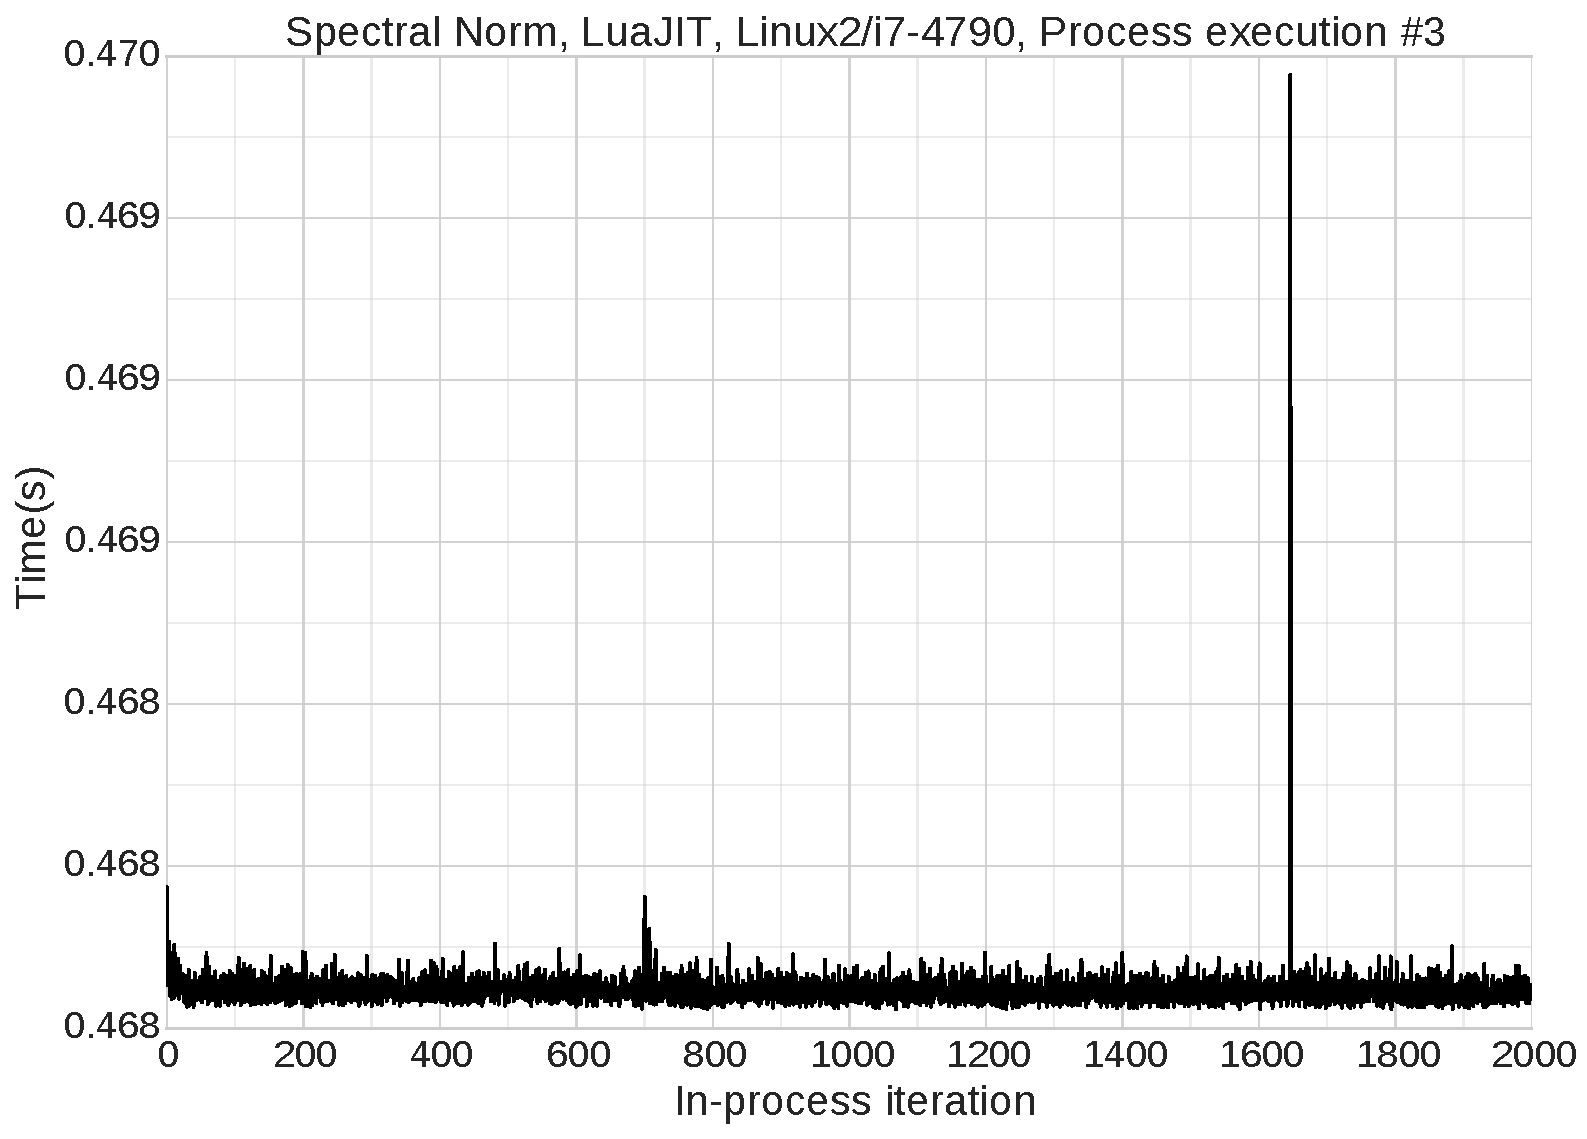
\includegraphics[width=.46\textwidth]{examples/outliers1}
\caption{Example of a benchmark with outliers.}
\label{fig:examples:outliers1}
\end{figure}


\subsection{Slowdowns}
\label{sub:slowdowns}

\sarah{This is one area were the sliding-window average might be useful (i.e. in detecting a slow-down).
One possible way forward would be to find a technique for performing hypothesis testing on time-series data, then running tests to determine whether the sliding-mean in one part of the chart is significantly different to the sliding-mean in an earlier phase of the execution.
This technique would also help to determine precisely when the warm-up phase is over and the JIT has kicked in.}
\cfbolz{this is a post-draft task}

A few benchmarks exhibit slow downs, where the first few iterations of a
benchmarks are faster than the eventual mean after ``warm up''.

Figure~\ref{fig:examples:slowdown1} shows one such example.

\begin{figure}[h!]
\centering
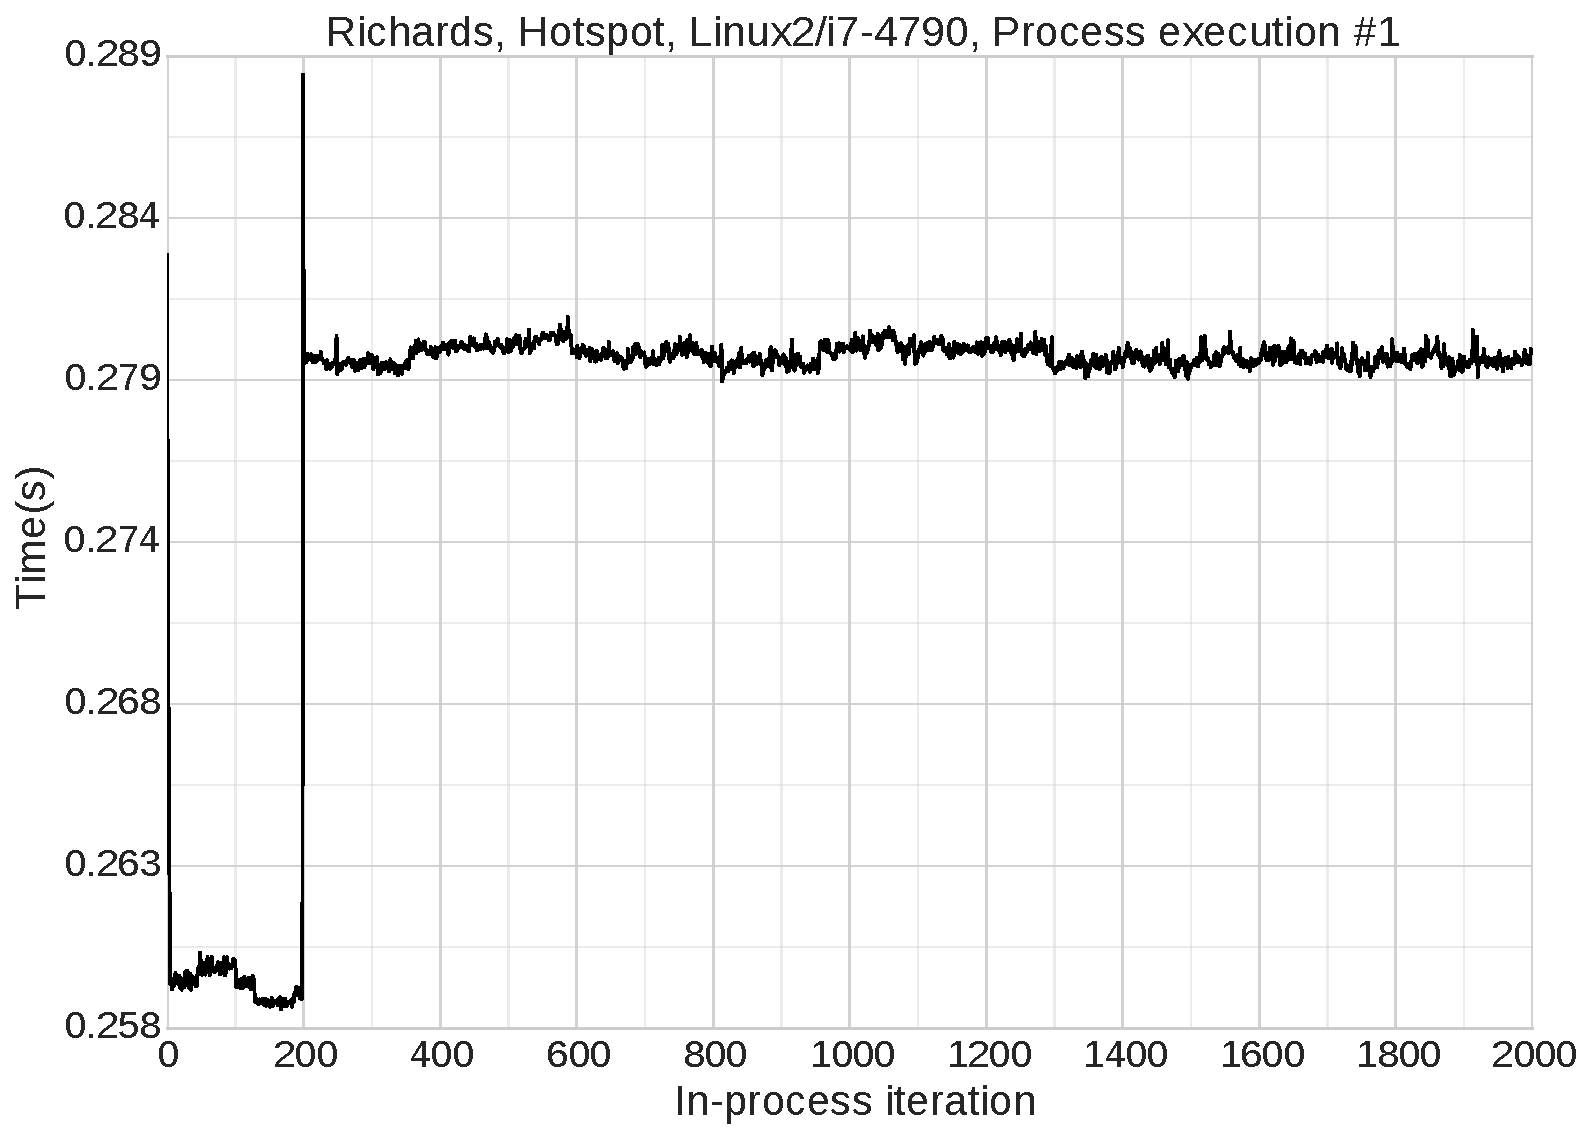
\includegraphics[width=.46\textwidth]{examples/slowdown1}
\caption{Example of a benchmark with a slowdown.}
\label{fig:examples:slowdown1}
\end{figure}



\subsection{Cyclic Behaviour}
\label{sub:cyclic}

Cyclic behaviour occurs in a number of benchmarks, which is a pattern of $n$
iterations that have similar timing results and keeps repeating across the
benchmark runs.

Figure~\ref{fig:examples:cycles1} shows one such example.

\begin{figure}[h!]
\centering
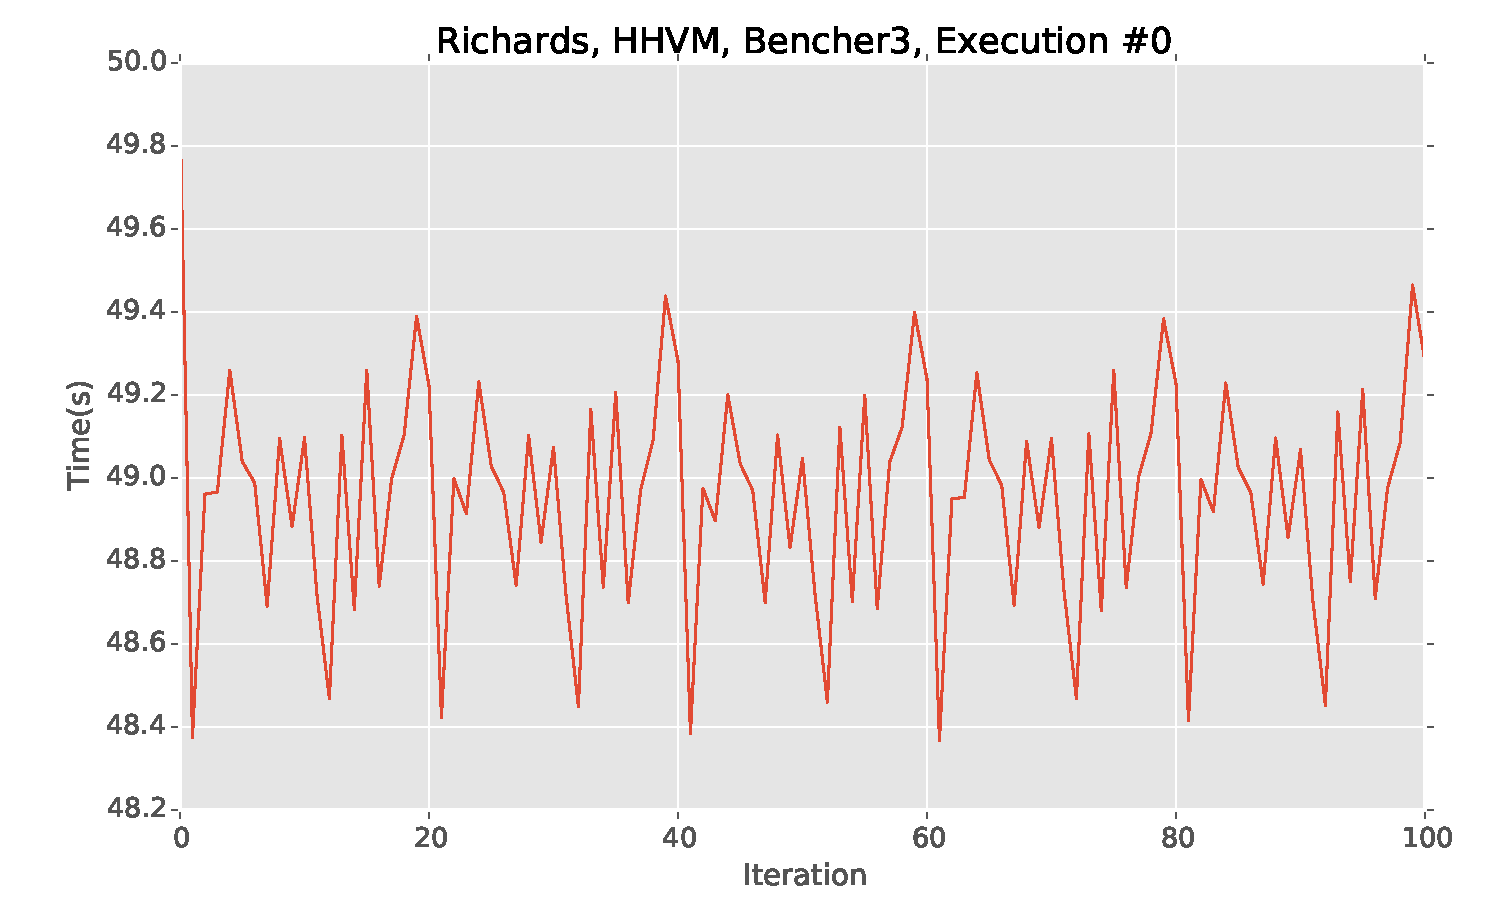
\includegraphics[width=.46\textwidth]{examples/cycles1}
\caption{Example of a benchmark with cycles.}
\label{fig:examples:cycles1}
\end{figure}


\subsection{Late Phase Changes}
\label{sub:phase}

Late phase changes occur in benchmarks where after many iterations the benchmark
changes behaviour, either by getting slower or faster, or by producing a
different pattern of randomness.

Figure~\ref{fig:examples:late1} shows one such example.

\begin{figure}[h!]
\centering
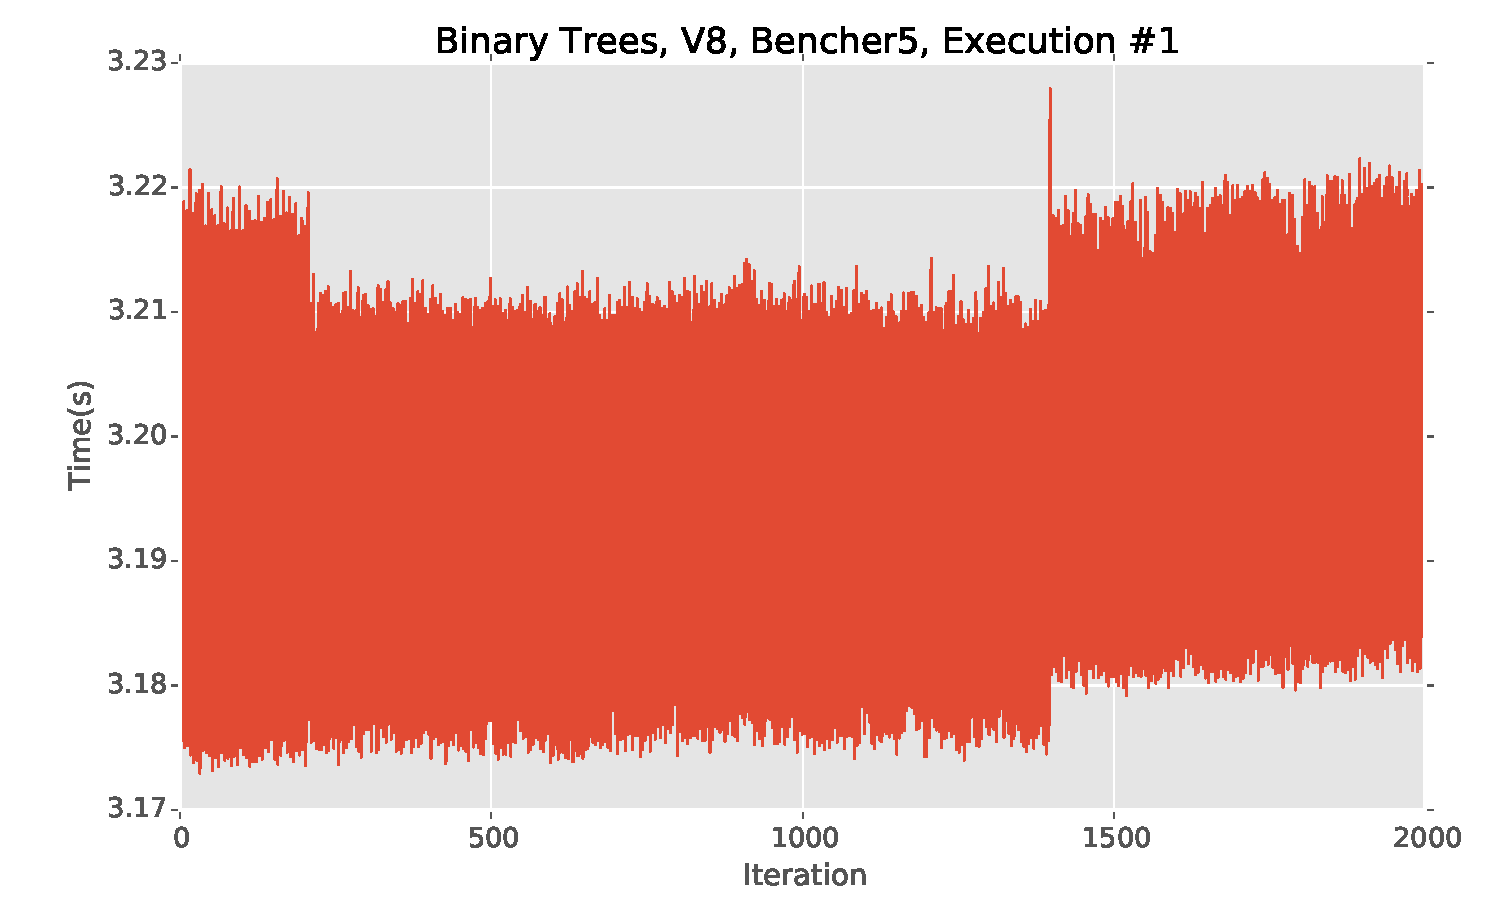
\includegraphics[width=.46\textwidth]{examples/late1}
\caption{Example of a benchmark with late phase changes.}
\label{fig:examples:late1}
\end{figure}


\subsection{Unexpectedly Long Warmup}
\label{sub:long}

The common understanding of warmup behaviour usually assumes that for such
small programs warmup is done after a few iterations. However, there are
benchmarks where performance improves after many hundred iterations.

\begin{figure}[h!]
\centering
\cfbolz{we need an example here}
\caption{Example of a benchmark with unexpectedly long warmup.}
\label{fig:examples:long}
\end{figure}

\subsection{Inconsistent Effects}
\label{sub:inconsistent}

A number of benchmarks have wildly different behaviour between different
iterations on the same machine, or between iterations of different machines.

Figure~\ref{fig:examples:consistent_weirdness1} shows a case where
unexpected behaviours are consistent between machines and executions.
Figure~\label{fig:examples:inconsistent_weirdness1} shows an example where
effects differ between both machines and executions.

\begin{figure*}[h!]
\centering
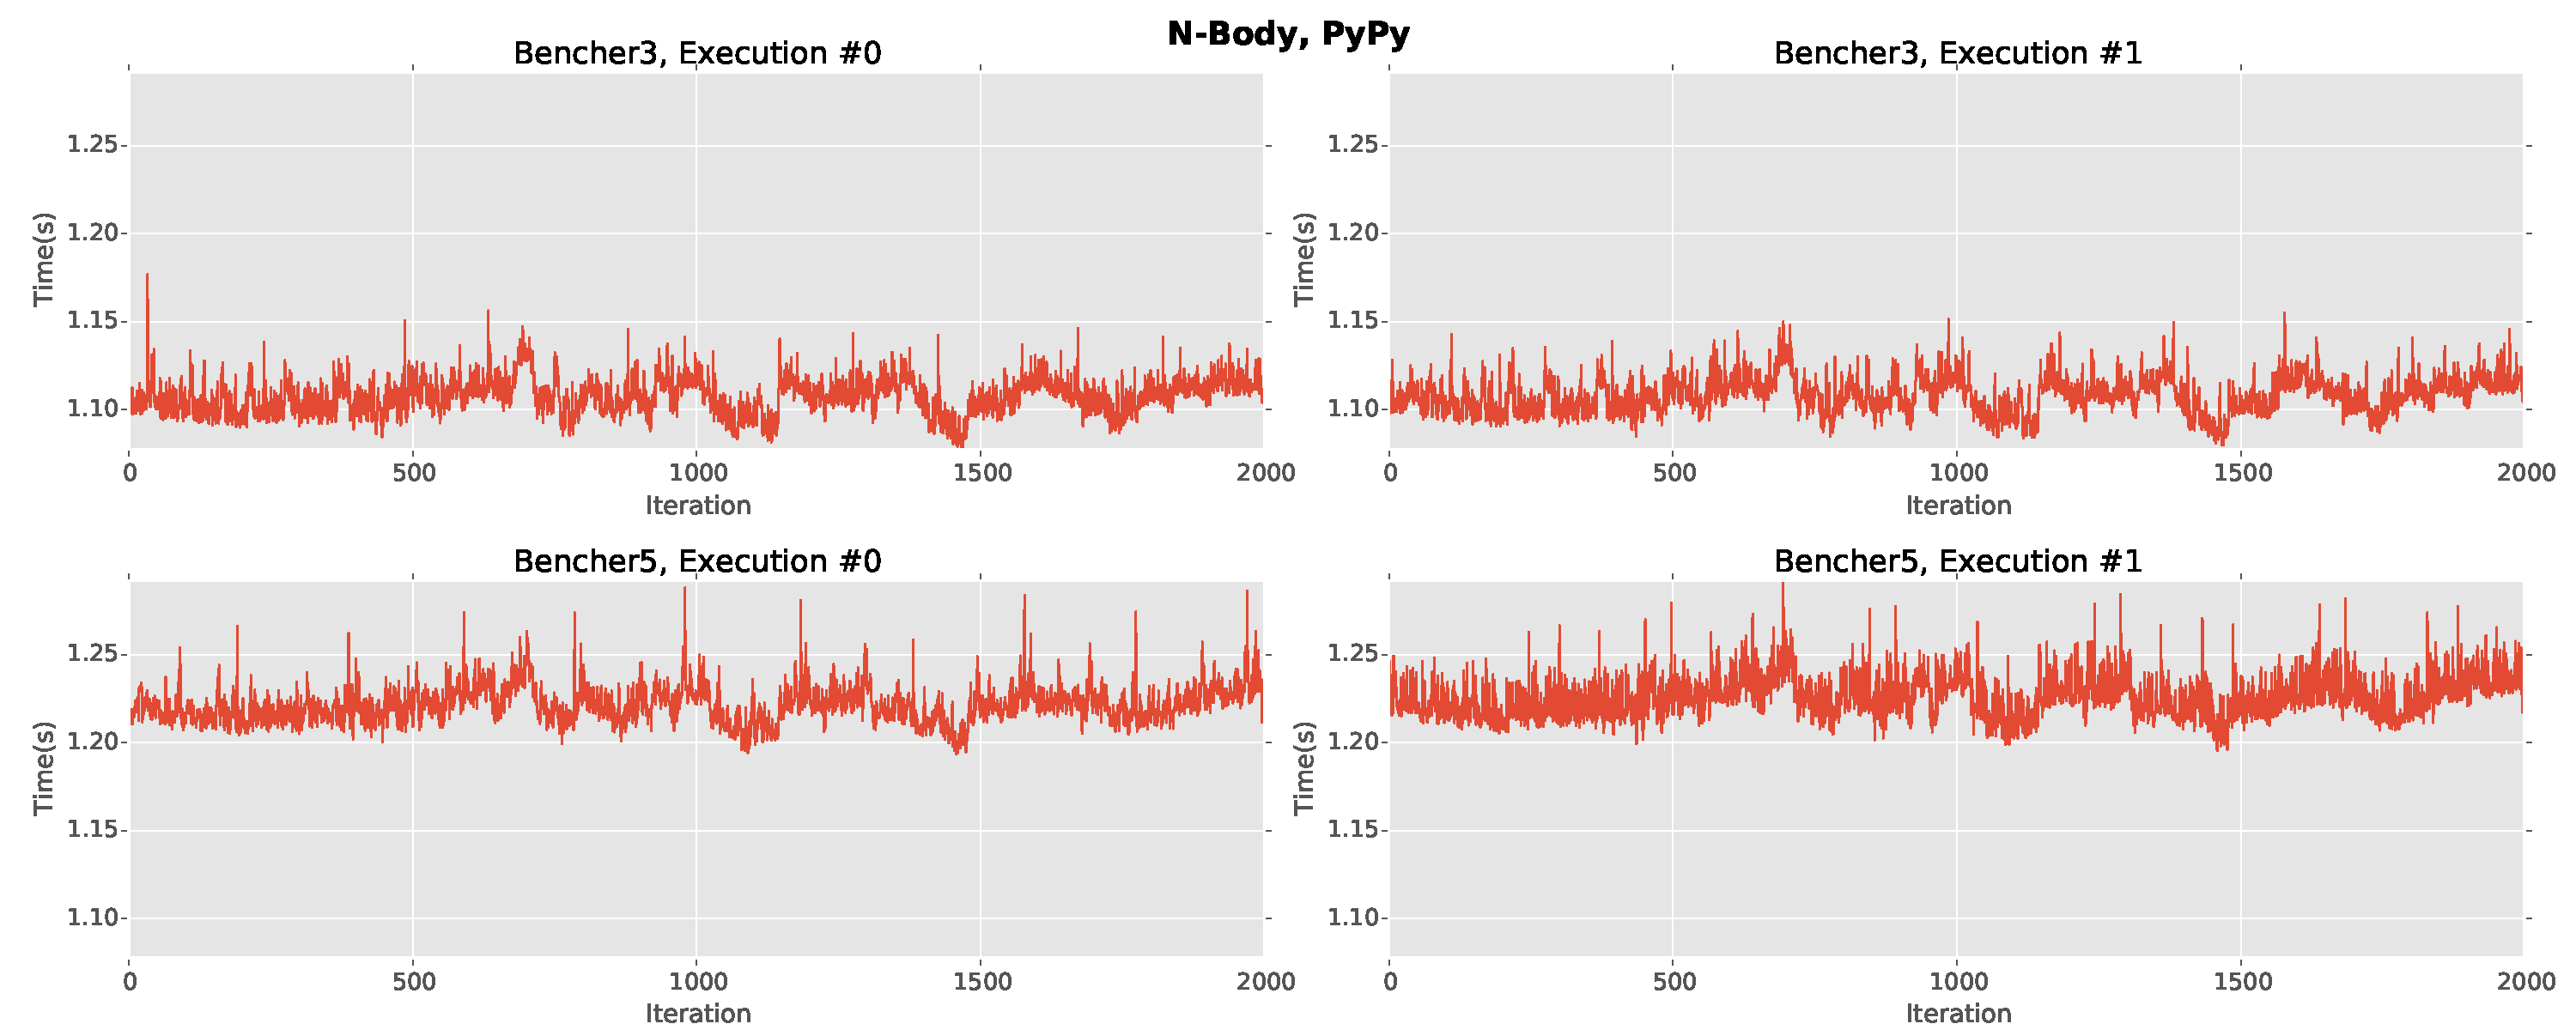
\includegraphics[width=\textwidth]{examples/consistent_weirdness1}
\caption{Example of a benchmark whose effects are consistent between machines and executions.}
\label{fig:examples:consistent_weirdness1}
\end{figure*}

\begin{figure*}[h!]
\centering
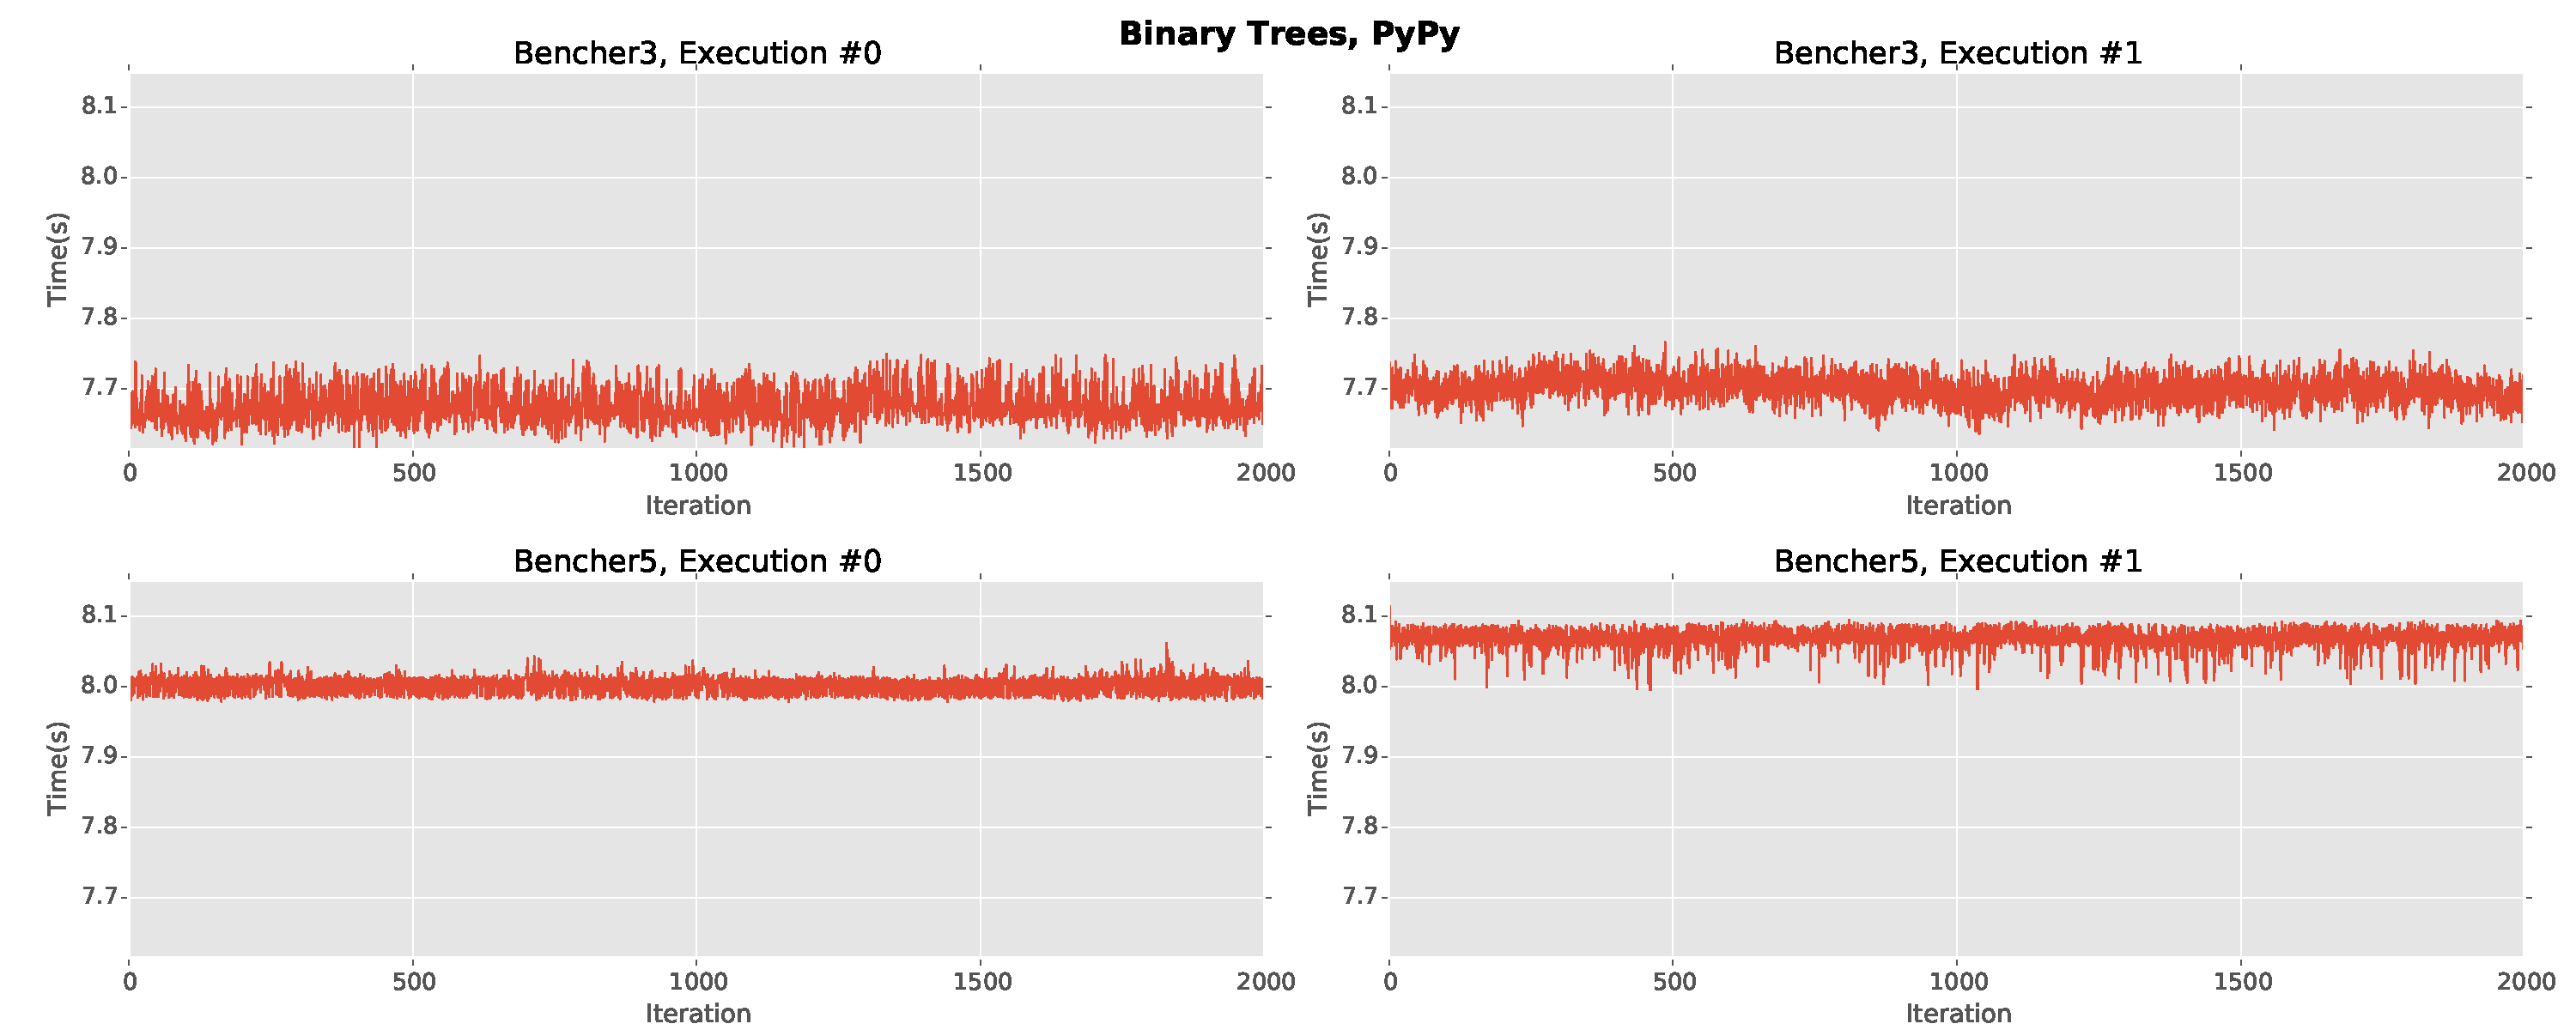
\includegraphics[width=\textwidth]{examples/inconsistent_weirdness1}
\caption{Example of a benchmark whose effects are inconsistent between machines and executions.}
\label{fig:examples:inconsistent_weirdness1}
\end{figure*}


\section{Threats to Validity}
\label{sec:threats}

\laurie{This is our best attempt at obtaining a constant CPU clock
speed. The Linux kernel documentation states that ``the idea that frequency can
be set to a single frequency is fiction for Intel Core
processors'':
\url{https://www.kernel.org/doc/Documentation/cpu-freq/intel-pstate.txt}}

While we have designed our experiment as carefully as possible, we do not
pretend to have controlled every possibly confounding variable. For example,
because of the large quantity of software we had to install, and because we used
different operating systems, we can not guarantee that the VMs were compiled in
precisely the same way on each machine. \laurie{if we're lucky, our cross-machine results
will be fairly stable, which will allow us to say something like ``despite the
possible variation across our machines, we got fairly stable results, suggesting
that this was not a significant issue in practise''.}

We use multiple different language implementations of benchmarks. Although our
checksums confirm that the different languages perform roughly the same work,
it is possible that some implementations may have an unfair advantage. This
could be due to the fact that some workloads are inherently easily optimised in
one language but not another, or perhaps because the original authors of the
benchmarks structured their code with optimisations in mind. An open question
is: should a multi-language benchmark suite should use idiomatic
implementations, implementations literally translated from a base version, or
the most performant implementations. Further it is not clear how having a
performance advantage impacts warmup characteristics.


\sarah{threats to validity: there may be some confounding variables that have
not been controlled in these experiments. There may be bugs in the JITs that
are being measured.  The benchmarks in the guest languages might be similar
enough that some important classes of behaviour have been missed, because the
benchmarks here do not trigger those behaviours.  There may be some un-thought
of explanation for weird JIT behaviour which has nothing to do with the JIT.}


\section{Related work}

There are two works we are aware of which explicitly note unusual warmup
patterns. Gil et al.'s main focus is on non-determinism over execution runs on
HotSpot, and the difficulties this raise in terms of providing reliable
benchmarking numbers~\cite{gil11microbenchmark}. In this process, they report at
least one benchmark (listBubbleSort) which on some executions undergoes what we
have termed warmdown \laurie{is that the term we're using?}. \kalibera note the
existence of what we have called cyclical behaviour, but require the user to
manually pick one part of the cycle for measurement~\cite{kalibera13rigorous}.


\section{Discussion}
\label{sec:Discussion}

  - discussion:
    - need to give up naive definition of warmup
    - unrealistic to get rid of these anomalies
    - some of benchmarking wisdom is wrong in the presence of this stuff
\sarah{Need some way to model the behaviour of JITs and perform hypothesis tests (so that people can answer questions like 'does this change in the VM actually make the JIT faster?').}

\section{Conclusions}
\label{sec:conclusion}

\bibliographystyle{abbrvnat}
\bibliography{bib}


\end{document}

